\documentclass{article}
\usepackage{fullpage}
\usepackage{amsmath}
\usepackage[margin=1in]{geometry}
\usepackage{graphicx}
\usepackage{xcolor}
\usepackage{float}
\usepackage{siunitx}
\usepackage{fancyhdr}
\usepackage{tcolorbox}
\usepackage{wrapfig}
\usepackage{lastpage}
\usepackage{listings}
\usepackage{tcolorbox}
\usepackage{mathabx}
\usepackage{wasysym}
\usepackage{physics}
\usepackage{verbatim}
\usepackage{color,soul}
\usepackage[utf8]{inputenc}


\tcbset{%
	colback=white,
	colframe=black,
	}

%Page formatting
\pagestyle{headings}
\setcounter{page}{1}
\pagenumbering{roman}

%Define colors for matlab lslisting at end of document
\definecolor{mygreen}{RGB}{28,172,0} % color values Red, Green, Blue
\definecolor{mylilas}{RGB}{170,55,241}
 
 %Lstlisting configuration
\renewcommand\lstlistingname{Algorithm}
\renewcommand\lstlistlistingname{Algorithms}
\def\lstlistingautorefname{Alg.}

%Matlab code formatting - change if you don't like the appearance for other coding languages or want specific color specifications
\lstset{language=Matlab,%
	%basicstyle=\color{red},
	breaklines=true,%
	morekeywords={matlab2tikz},
	keywordstyle=\color{blue},%
	morekeywords=[2]{1}, keywordstyle=[2]{\color{black}},
	identifierstyle=\color{black},%
	stringstyle=\color{mylilas},
	commentstyle=\color{mygreen},%
	showstringspaces=false,%without this there will be a symbol in the places where there is a space
	numbers=left,%
	numberstyle={\tiny \color{black}},% size of the numbers
	numbersep=9pt, % this defines how far the numbers are from the text
	emph=[1]{for,end,break},emphstyle=[1]\color{red}, %some words to emphasise
	%emph=[2]{word1,word2}, emphstyle=[2]{style},    
}

%Indenting and skipping length settings - can adjust for formatting needs
\setlength{\parindent}{0.0in}
\setlength{\parskip}{0.05in}

% Edit these values as appropriate
\newcommand\course{ENAE 483}
\newcommand\hwnumber{1}                  % <-- homework number
\newcommand\NetIDa{Abdullah Alnamlah, Joseph Hauerstein,\\ Emma Perez, Mahek Shah,\\ Anderson Romero}           

%Pagestyle setup
\pagestyle{fancyplain}
\headheight 35pt
\lhead{\NetIDa}
%\lhead{\NetIDa\\\NetIDb}                 % <-- Comment this line out for problem sets (make sure you are person #1)
\chead{\textbf{\Large Submission \hwnumber}}
\rhead{\course \\ \today}
\lfoot{}
\cfoot{}
\rfoot{\small\thepage}
\headsep 1.5em

\renewcommand{\thesubsection}{\thesection.\alph{subsection}}

\begin{document}

%Problem structure recommended to follow within the \section and \subsection and \subsubsection(cont...) structure for problems and subparts of problems
\section{Flow Chart}

%\subsection{} \label{YouCanLabelSectionsandSubsections}

%Also with a box around it
%\begin{tcolorbox}
%Alternate unit formatting: \SI{11.3892}{kg m^2 s^{-1}}
%\end{tcolorbox}



%General format for a figure - change the width value to adjust picture size
\begin{figure}[H]
    \centering
    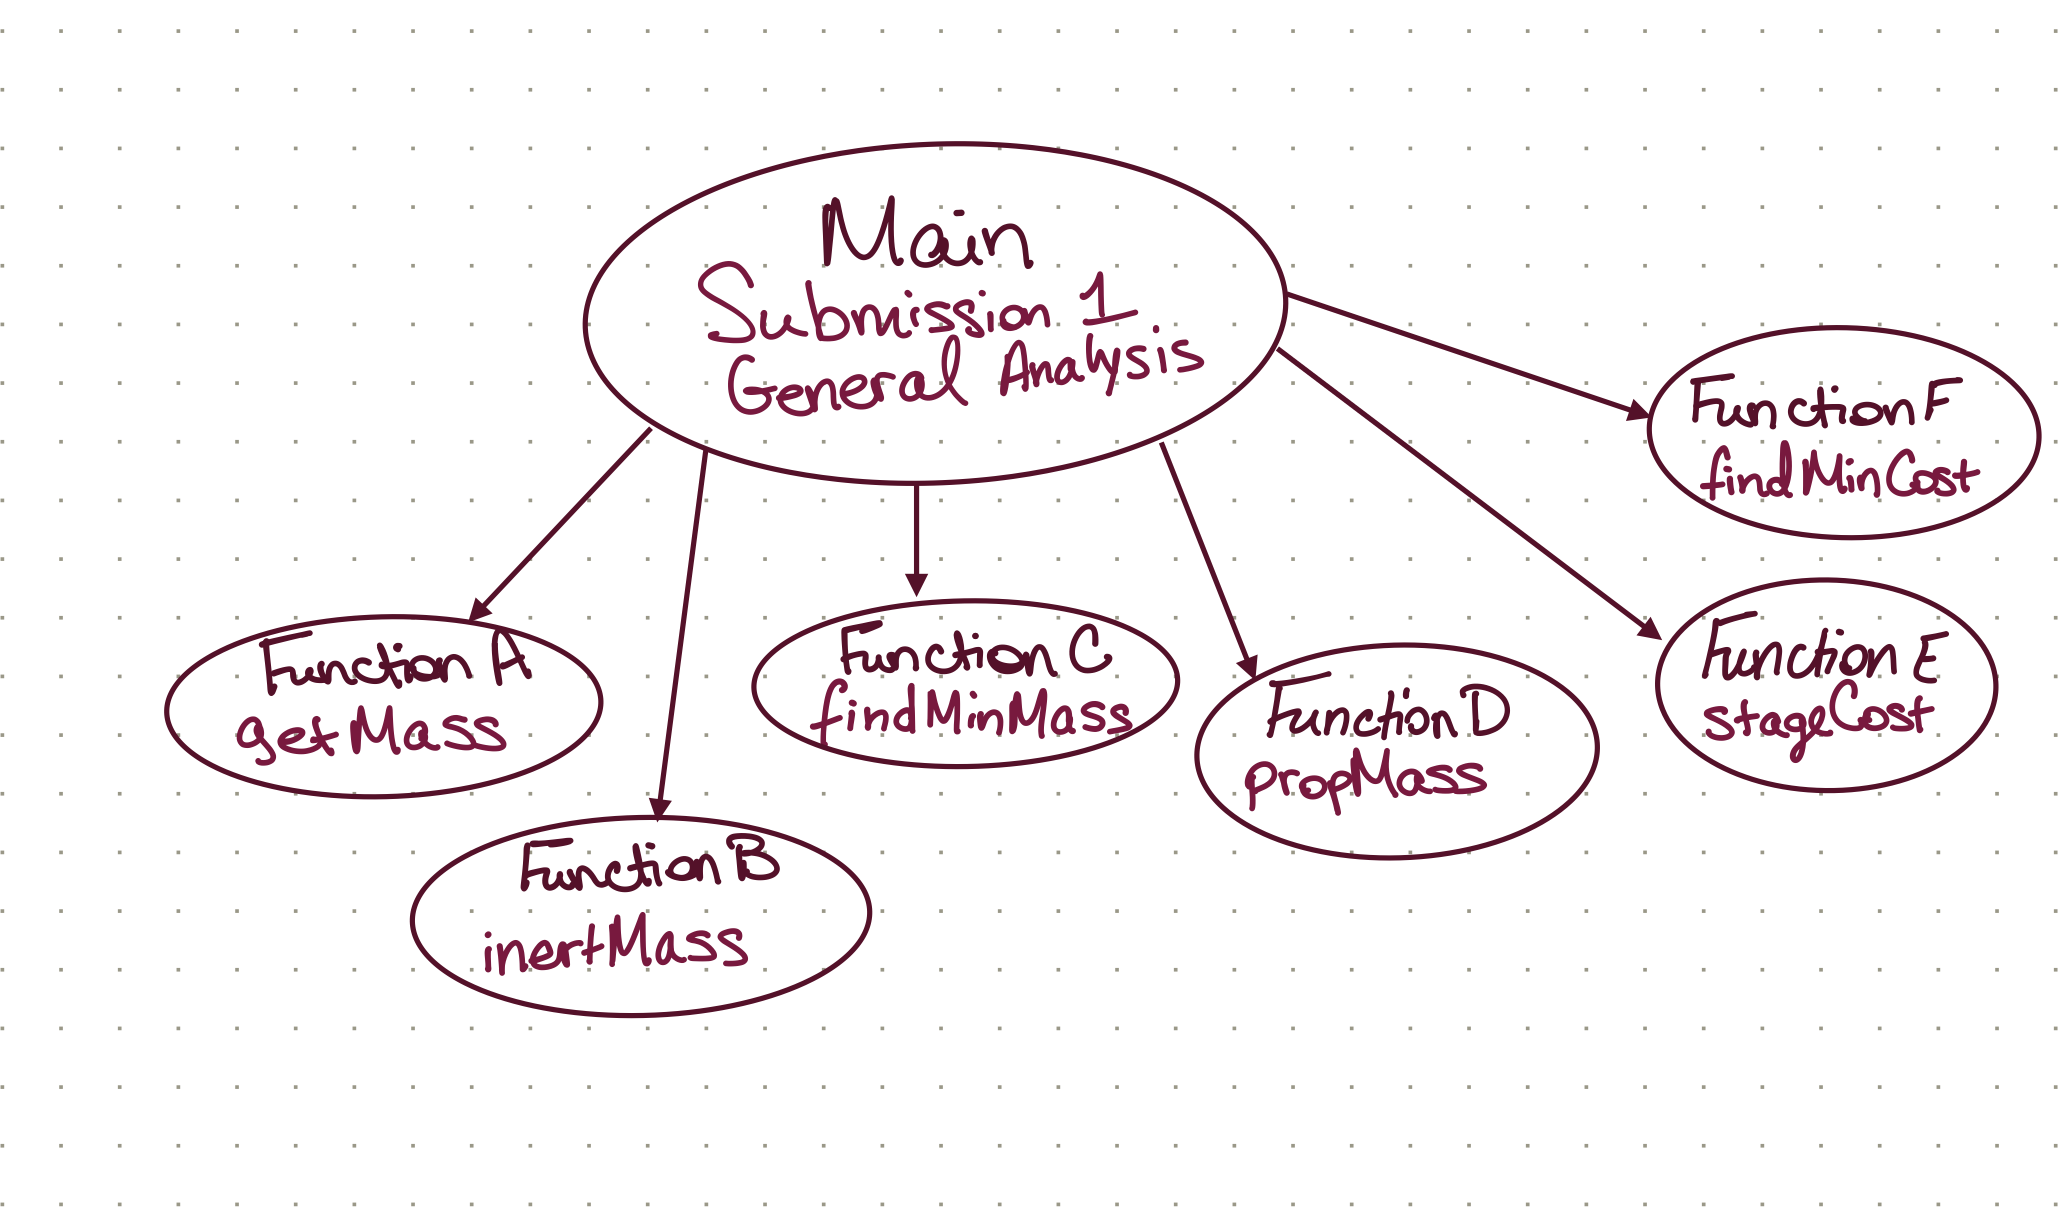
\includegraphics[width=0.65\textwidth]{./main_flow_chart.png}
    \caption{Flow Chart of Function Organization}
    \label{fig: main_flow_chart}
\end{figure} 

\begin{figure}[H]
    \centering
    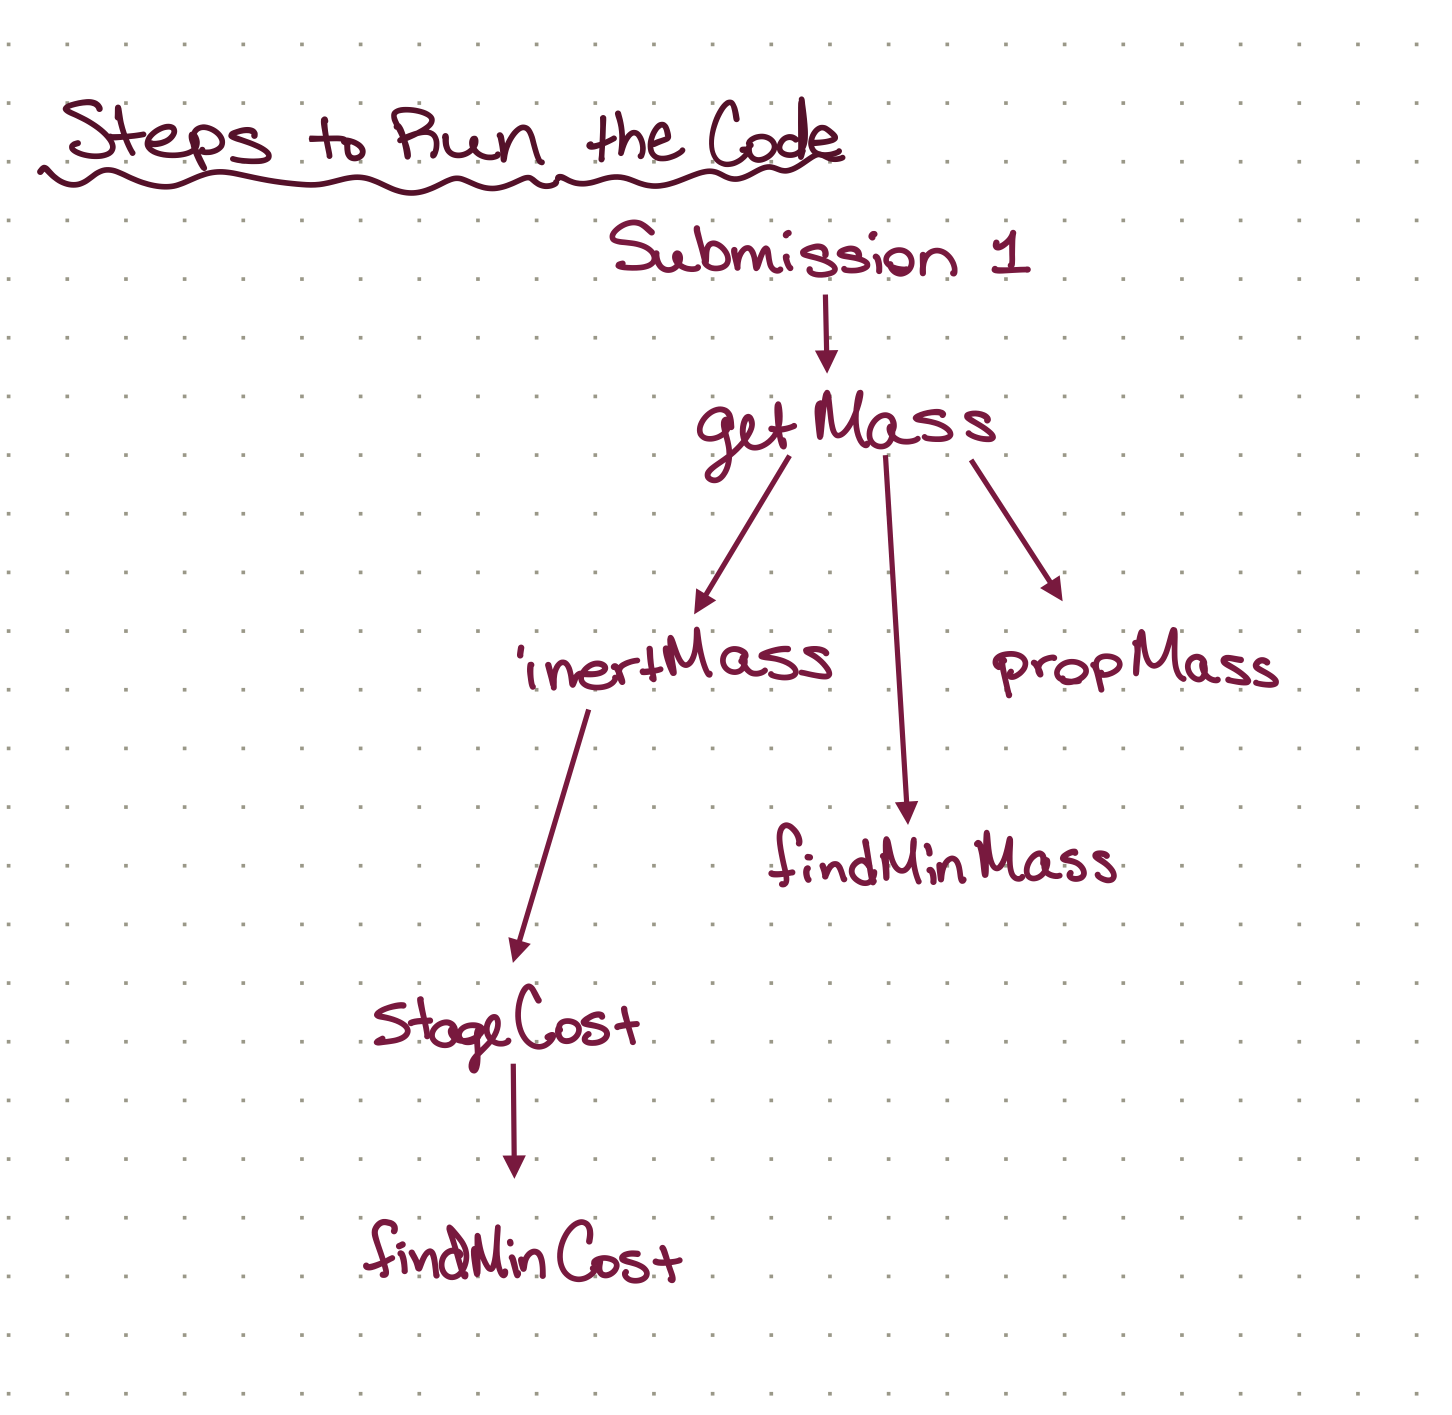
\includegraphics[width=0.65\textwidth]{./steps_to_run.png}
    \caption{Flow Chart of Function Call Order}
    \label{fig: steps_to_run}
\end{figure} 


%An equation:
%\begin{equation} \label{eq:2BP}
%    \Ddot{\Vec{r}} = \frac{-\mu}{r^3}\Vec{r}
%\end{equation}

%An unnumbered equation:
%\begin{equation*} \label{eq:2BP}
%    \Ddot{\Vec{r}} = \frac{-\mu}{r^3}\Vec{r}
%\end{equation*}



%An example of what matlab code might look like after it has been uploaded
\newpage
\section{Code}
\lstinputlisting[language=matlab]{../src/joseph_1_2.m}
\lstinputlisting[language=matlab]{../src/getMass.m}
\lstinputlisting[language=matlab]{../src/inertMass.m}
\lstinputlisting[language=matlab]{../src/propMass.m}
\lstinputlisting[language=matlab]{../src/findMinMass.m}
\lstinputlisting[language=matlab]{../src/stageCost.m}
\lstinputlisting[language=matlab]{../src/findMinCost.m}

\end{document}